\section{Checkpointing} \label{sec:2-5-bg-checkpointing}
In this section, I will show how to reduce the peak memory established in the previous section using checkpointing and motivate my extension to Gruslys et al.'s technique \cite{Gruslys2016}.
% The first key behind all memory optimisations using this graph is that the entire training process is this exact same step repeated many times.
% Thus, even though training may take days or even weeks [?], we only have to optimise a relatively small computational graph.
% Compared to the time taken for a single training step, we can spend a huge amount of time solving for the best optimisation strategies; it only has to be fast relative to the entire training process.


% something about redsicovered from AD
%%%%%%%%%%%%%%%%%%%%%%%%%%%%%%%%%%%%%%%%%%%%%%%%%%%%%%%%%%%%%%%%%%
\subsection{\texorpdfstring{\(\Theta(\sqrt{N})\)}{\textit{O(sqrt(N))}} Checkpointing}
Consider the simplified computational graph of backpropagation that was derived in the previous Section \ref{sec:2-4-memory-analysis}, or more generically, the graph for computing the adjoint of a sequence of operations.
I have shown this to have linear space complexity in Section \ref{sec:2-4-memory-analysis}, due to the forwards being stored for use in the backwards pass.
We can elide this restriction by trading off compute for memory, using what is known as \textit{checkpointing}.

In checkpointing, only some of the forwards are stored in memory, known as the checkpoints, or snapshots.
Then, during the backwards pass, forwards are recomputed from the last checkpoint in the chain, this time keeping them in memory so the backwards pass can proceed.
Thus, the checkpoints have split the sequence into segments, and
to \textit{compute the adjoint of the entire sequence}, we first run the forward pass only storing the checkpoints (which demaracte the segments),
then proceed backwards by \textit{computing the adjoints segment-by-segment},
where computing the adjoint of a segment involves recomputing the forwards from the last checkpoint and this time storing them in memory so the adjoint can proceed.
This segmented backwards pass is visualised in Figure \ref{fig:2-backprop-segmented}, repeated from the introduction.

\begin{figure}[h]
    \centering
    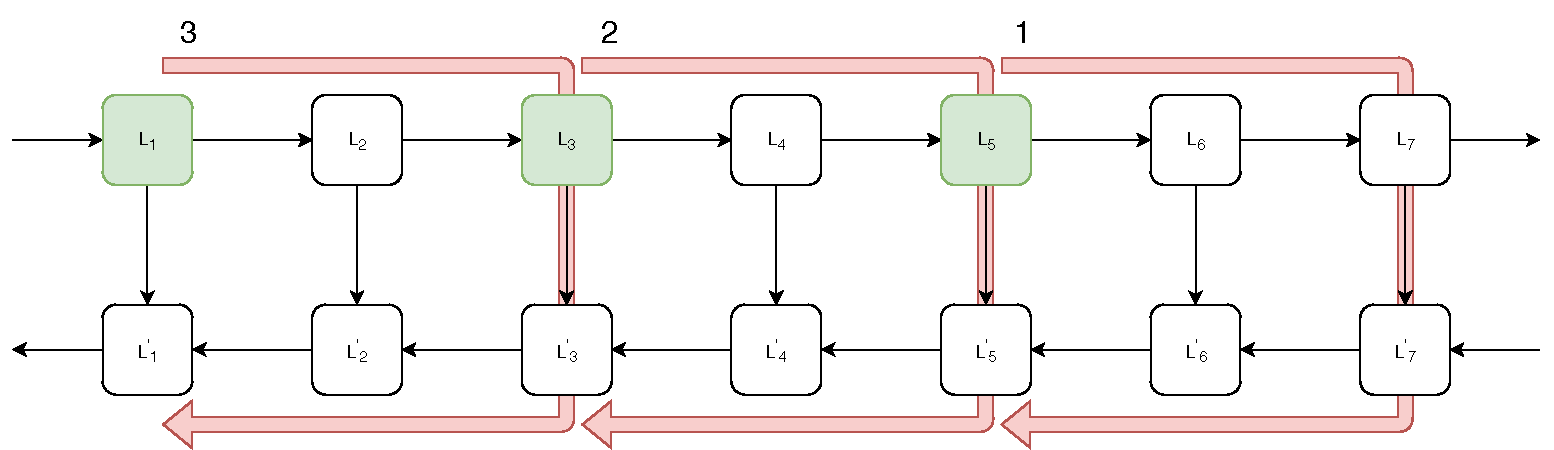
\includegraphics[width=0.92\linewidth]{backprop_segmented.pdf}
    \caption{Segmented backpropagation with checkpointing: Say we are computing the backward pass. The forward pass has already been computed, and only the outputs of \(L_1\), \(L_3\), and \(L_5\) were stored. Then, to perform the backward pass, we perform backproagation (both forward and backward) for segments 1, then 2, then 3, as shown.}
    \label{fig:2-backprop-segmented}
\end{figure}

Assuming uniform per-operator costs, the new peak memory requirement still occurs at the end of the chain, but is now lowered to only the cost of the checkpoints, rather than the entire forward sequence, plus the cost of computing the adjoint of the final segment.
Assuming \(k-1\) checkpoints that split the sequence of length \(n\) into \(k\) evenly-sized segments, the peak memory cost is approximately:
\begin{equation*}
    g(n) \;=\; \Theta(\sfrac{n}{k}) + \Theta(k)
\end{equation*}
With basic calculus, it can be found that \(k = \sqrt{n}\) minimises this, with a sublinear cost of \(2\sqrt{n}\).
As every forward is recomputed at most once, the computational overhead is no more than the cost of a single extra forward pass.
According to Chen \cite{Chen2016}, the forward pass is about twice as fast as the backward pass, resulting in the actual overhead being around 30\%.

%%%%%%%%%%%%%%%%%%%%%%%%%%%%%%%%%%%%%%%%%%%%%%%%%%%%%%%%%%%%%%%%%%%%%%%%%%%%%%%%
\subsection{Multiple Recomputations}
The peak memory cost can be reduced even further by introducing \textit{multiple recomputations}.
The above technique split the adjoint computation of a sequence into the adjoint computations of segments of this sequence.
There is no reason that, during the adjoint computation of a segment, we cannot recursively apply the technique by splitting the segment into sub-segments.

That is, consider the scenario where the forward pass of the sequence has been computed and we are now processing a segment.
We compute the forwards of the segment (their first recomputation), storing only some checkpoints. Then we perform the adjoint computation on each sub-segment, resulting in the dropped forwards being recomputed a second time. We could keep recursively applying the technique on the sub-segments resulting in many recomputations.

A visualisation of how we move forwards and backwards along a sequential computation during multiple recomputations is shown in Figure \ref{fig:2-multiple-recomps-vis}.

\begin{figure}[h]
    \centering
    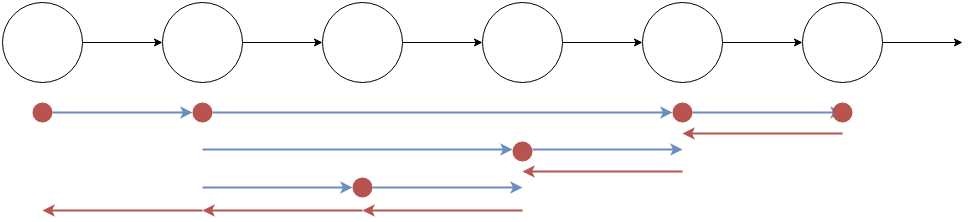
\includegraphics[width=0.8\linewidth]{multiple_recomps_vis.png}
    \caption{Execution of multiple recomputations on a sequence. Blue arrows represent forward computation. Red arrows represent backward computation. Red circles denote a forward being checkpointed. Moving vertically down represents the next recursion depth - blue arrows on the \(i^{\mathrm{th}}\) line are being computed for the \(i^{\mathrm{th}}\) time, or recomputed for the \({i-1}^{\mathrm{th}}\) time.}
    \label{fig:2-multiple-recomps-vis}
\end{figure}

When applying this recursive scheme, always storing \(k\) evenly-spaced checkpoints per segment, the peak memory cost becomes the cost of the \(k\) checkpoints plus the (recursive) cost of one segment:
\begin{equation*}
    g(n) \;=\; k + g(\sfrac{n}{k+1})
\end{equation*}
Solving this gives:
\begin{equation*}
    g(n) \;=\; k\log_{k+1}(n)
\end{equation*}
Setting \(k\,=\,1\) minimises this to \(\log_2(n)\). \todo{EXPLAIN COMP COMPLEXITY}
Setting up a similar recurrence for the computational cost shows it has increased to \(n\log_k(n)\).
This demonstrates how, through multiple recomputations, we have further traded compute for memory.

Going beyond this recursive formulation, the extreme case of simply `recomputing everything' gives \(\Theta(\mathrm{1})\) memory at \(\Theta(n^2)\) computational cost:
Say we have the forward at the start of the chain, \(f_0\), and the backward at the end, \(b_n\);
we compute the forwards in-place, from \(f_0\) to \(f_{n-1}\), then use that and \(b_n\) to compute \(b_{n-1}\).
Thus, we have done one step of the backwards pass in \(\Theta(\mathrm{1})\) space.
To perform the next step, we simply repeat this process, computing in-place \(f_0\) to \(f_{n-2}\) and using \(b_{n-1}\) to get \(b_{n-2}\), and so on until we have \(b_0\), still only using \(\Theta(\mathrm{1})\) space. The computational overhead is quadratic because the first forward pass is over \(n\) steps, then the second \(n-1\) steps, then \(n-2\) steps, and so on. Summing these gives \(\Theta(n^2)\).

%%%%%%%%%%%%%%%%%%%%%%%%%%%%%%%%%%%%%%%%%%%%%%%%%%%%%%%%%%%%%%%%%%%%%%%%%%%%%%%%
\subsection{Limitations of Checkpointing Techniques and their Implementations}
Griewank first proposed all of these techniques for sequential adjoint computations in 1992 \cite{Griewank1992}, later developed into the \texttt{REVOLVE} algorithm with Walther \cite{Revolve2000}.
Given a fixed number of checkpoints per recomputation pass and the sequence length, it solves for a strategy that uses the least recursion depth (the max number of recomputation passes).
For a recursion depth of \(r\) and number of checkpoints \(s\), a sequence of length \(\binom{s+r}{r}\) can be executed in logarithmic space, where \(\binom{\cdot}{\cdot}\) is the binomial coefficient.
However, their work assumes uniform per-operator costs.
A lot of AD literatature is in the domain of differential equations on time, where such assumptions may hold, but it is not the case for most neural networks.

Martens and Sutskever \cite{Martens2012} briefly outlined the (uniform costs) \(\sqrt(n)\) technique for neural networks in 2012.
Chen made the technique more widely known with his 2016 paper \cite{Chen2016} and corresponding implementation in MxNet \cite{mxnet-memonger}.
It has since been implemented in PyTorch \cite{torch-memonger} and TensorFlow \cite{openai-checkpointing}.
Chen also presented the asymptotic analysis for the recursive scheme and gave an algorithm that, given the original (arbitrary) computational graph and the number of times to recompute each individual forward, will construct a new graph that performs the adjoint computation according to this policy, using `node mirroring'.

Though these techniques greatly reduce the memory cost by trading off computation, they pick an arbitrary point on the compute-memory trade-off curve.
That is, given infinite memory, we could of course do any computation with no overhead, as we would simply not use checkpointing.
However, as the memory budget is tightened, we are forced to checkpoint, incurring compute overhead.
Ideally, the user should specify their memory budget and the system should find the checkpointing strategy that satisfies this budget with the least computational cost, rather than having the user specify arbitrary parameters like the number of checkpoints.
They should not even have to know what checkpointing is.

Chen proposed a heuristic algorithm that, given the memory budget and per-operator memory costs, traverses the sequence and greedily chooses to drop nodes until the cost of that segment exceeds the budget, at which point the current node is instead checkpointed, starting a new segment.
To try to match the memory savings of \(\sqrt{n}\) checkpointing for sequences with abitrary per-operator costs, another heuristic is used for guiding a grid search over the memory budget to find the plan returned by the algorithm that gives the least memory cost.
Though this does not give the provably optimal memory cost, they do report good results.
However, the more important limitations are that this is restricted to one recomputation and that it makes no attempt to optimise for computational cost, only to minimise the memory cost.

Again, ideally, we want to solve for the optimal checkpointing policy that (i) minimises computational cost whilst satisfying a memory budget, and (ii) does so according to the precise per-operator compute and memory costs. 

Before detailing Gruslys et al.'s \cite{Gruslys2016} work on memory-efficient RNN training, which achieves the former goal but not the latter, I will briefly discuss some related work on checkpointing.

%%%%%%%%%%%%%%%%%%%%%%%%%%%%%%%%%%%%%%%%%%%%%%%%%%%%%%%%%%%%%%%%%%%%%%%%%%%%%%%%
\subsection{Related Work}
\todo{TODO} This section should either be much more in-depth or removed.

\texttt{REVOLVE} gives the optimal recursion depth for sequences of known length.
Work has also been done for sequences of unknown length.
\texttt{REVOLVE}'s optimality has been matched for sequences that do not exceed a length that has a certain bound with respect to the number of checkpoints per segment.
Some deep learning models, like \texttt{seq2seq} RNNs, do have unknown sequence length, so there could be some opportunity here.
However, I only consider sequential neural networks where the sequence length is known.

Dauvergne and Hasco\"{e}t reframe checkpointing in terms of the data-flow equations used in compilers \cite{Dauvergne2006}.
They also formalise what other data-flow techniques from compilers look like for automatic differentiation, such as liveness analysis and \textit{to be recorderd} analysis, and seek to combine them with checkpointing in their \texttt{TAPENADE} platform.

Siskind and Pearlmutter \cite{Siskind2018} generalised \texttt{REVOLVE} to arbitrary computation \textit{trees}, rather than just sequences.
However, their implementation does not take into account precise per-operator costs and does not solve for the least computational cost given a memory budget, but instead gives \texttt{REVOLVE}-like optimality by finding the strategy of least recursion depth.
Also, though non-linear architectures are now prevalent in neural networks, they tend to not be trees either.

\todo{others} H-revolve? Imperial one? Those two new papers that generalise to arbitrary graphs?
% heirarchical checkpointing: async and sync? num levels of memory? Assumptions on comp costs, memory costs, transfer costs, allocation costs?

\subsection{Optimal Compute Cost Checkpointing Through Dynamic Programming}
% 5. DeepMind
% Finally something that gives optimal C for bounded B
% Only for uniform cost RNNs
% explain RNN cell and how they interpret `memory slots'
% DP eqns and algo
% Base cases: do in-place, do drop everything
% rec case: forwards to k, right storing k, left
% Policy can then be `traversed'
Gruslys et al. solve for the checkpointing policy that gives the least computational cost, subject to a memory budget \cite{Gruslys2016}.
They formulate this as a dynamic programming (DP) problem where the subproblems are over the sub-sequences and the size of the memory budget.
The solution is defined for RNNs, where every layer in the sequence is an identitical RNN \textit{cell}, leading to uniform per-layer costs.
The first implication of this is that they can talk about memory in terms of `memory slots' instead of precisely-sized buffers, where one slot is a workspace for everything needed to compute the forwards and backwards of one cell.
Similarly, computational cost can be described using arbitrary units.
Secondly, every sub-sequence of length \(t\) is identitical, so there is no need to solve subproblems for all possible subsequences, but only over sequences of length \(1\leq t\leq n\).

The problem is formulated similarly to how Markov Decision Processes are optimised in Reinforcement Learning \cite{Bellman1954, Sutton1998}.
There is a cost function for states \(C(t, m)\), where a state is a pair of the sequence length \(t\) and the number of memory slots \(m\).
This returns the least computational cost achievable for that pair.
\(C(t, m)\) is defined recursively on the subproblems for smaller sequences and fewer memory slots.
There is a policy \(D(t, m)\) that says for each state what action should be chosen - that is, what layer should next be checkpointed. \(1 \leq y < t\) denotes the action and is defined as the offset to the next layer to be checkpointed.
The cost \(C(t, m)\) of a state depends on what the policy says we should do in that state.
The cost-action function \(Q(t, m, y)\) is the cost of the state \((t, m)\) if we choose action \(y\).

Thus, to find the optimal \(C(t, m)\) we must know the optimal costs for all the subproblems, so we can choose the action \(y\) that gives the optimal cost for this problem.
We therefore need to co-optimise these mutually recursive functions, which are defined as follows:
\begin{align*}
    C(t,\, m)      \;&=\; Q(t,\, m,\, D(t,\, m))\\[0.5em]
    Q(t,\, m,\, y) \;&=\; \text{some function of } y \text{ and relevant subproblems } C(t\prime,\, m\prime)\\[0.5em]
    D(t,\, m)      \;&=\; \argmin_{1\leq y < t}\, Q(t,\, m,\, y)
\end{align*}
This can be solved using standard DP techniques. Gruslys et al. use bottom-up value iteration.
I will give the algorithm after fully describing the solution.

That is, the base cases of \(C\) and the recursive case \(Q\) that actually solve our original problem: finding the least computational cost within which we can perform backpropagation on a sequence of length \(t\) whilst satisyfing the memory budget \(m\), using checkpointing.

First, the base cases. 
For \(C(1, m)\), we simply perform the forwards and backwards for that single cell, giving a cost of 1.
For \(C(t, 1)\), we use the \(\Theta(1)\) space technique discussed above that recomputes everything, resulting in a quadratic cost.
For \(C(t, m)\) where \(m \geq t\), there is enough memory to not do any checkpointing, resulting in linear computational cost.

\begin{figure}[thb]
    \centering
    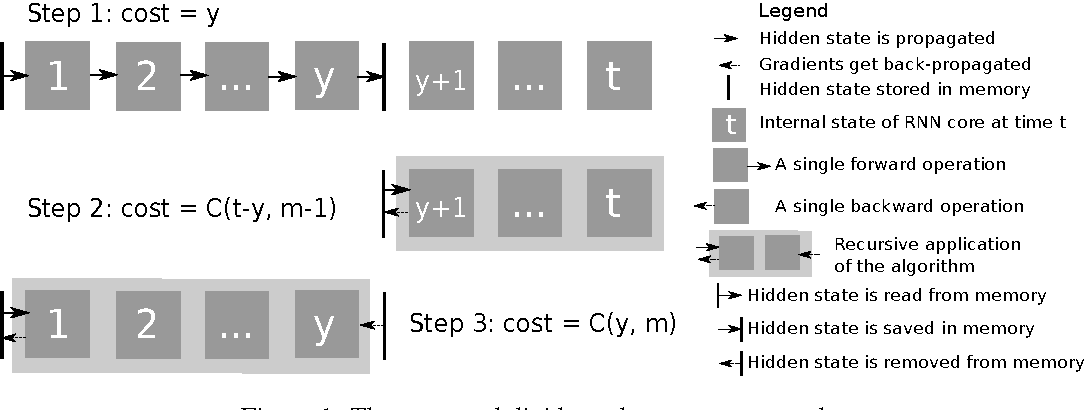
\includegraphics[width=0.97\linewidth]{dp-checkpointing-recursive-case.png}
    \caption{The recursive case \(Q(t, m, y)\): computing the forwards to \(y\), recursing on the right whilst storing \(y\), and recursing on the left with all the slots \cite[Figure~1]{Gruslys2016}. `hidden states' refer to the forwards.}
    \label{fig:2-dp-checkpointing-rec}
\end{figure}

The recursive case can be formulated as shown in Figure \ref{fig:2-dp-checkpointing-rec}, taken from the original paper\footnote{This is spcifically for BPTT-HSM, where the hidden states are checkpointed. See the paper for more details.}.
For \(Q(t, m, y)\), we first compute the forwards up to \(y\) without storing them, incurring a compute cost of \(y\).
Then, we recurse on the right hand side holding \(y\) in a memory slot.
That means we are recursing on a sequence of length \(t-y\) with \(m-1\) slots.
Once this returns, we can recurse on the left hand side.
The left sequence is of length \(y\) and we can use all \(y\) slots, because the forward of \(y\) is not required to backpropagate on the left hand side.
Thus, the cost-action function is defined as:

\begin{equation*}
    Q(t,\, m,\, y) \;=\; y \,+\, C(t\,-\,y,\, m\,-\,1) + C(y,\, m)
\end{equation*}

The algorithm for solving these equations is given in Algorithm \ref{alg:2-policy-solver}.
I do not explicity define the linear cost base case as it depends on whether you are storing the full internal state of an RNN cell or just the hidden state and recomputing the internal state.
I do not dwell on this further as I will be extending the technique for general feedforward networks where this is not a consideration.

The algorithm is bottom-up:
It first sets the base cases, before moving `up' through the search space, solving for longer sequences and more memory slots recursively.
The recursive case chooses the \(y\) that gives the least \(Q(t,\, m,\, y)\).
It sets \(C(t,\, m)\) to that cost and \(D(t,\,m)\) to \(y\).

\begin{algorithm}[h]
\DontPrintSemicolon
\KwIn{\(t_{max}\) the maximum sequence length}
\KwIn{\(m_{max}\) the maximum memory capacity}
\BlankLine

Let \(C\), \(D\) be 2D arrays of size \(t_{max}\times m_{max}\)\;
\For{\(t \,\in\, \{1,\,\ldots,\,t_{max}\}\)}{
    \(C[t][1] \;\leftarrow\; \frac{t(t+1)}{2}\)\;
    \For{\(m \,\in\, \{t,\,\ldots,\, m_{max}\}\)}{
        \(C[t][m] \;\leftarrow\;\) \textit{linear cost}\;
        \(D[t][m] \;\leftarrow\; 1\)\;
    }
}
\BlankLine
\For{\(m \,\in\, \{2,\,\ldots,\, m_{max}\}\)}{
    \For{\(t \,\in\, \{m+1,\,\ldots,\,m_{max}\}\)}{
        \(C_{min} \;\leftarrow\; \infty\)\;
        \For{\(y \;\in\; \{1,\,\ldots,\,t-1\}\)}{
            \(c \;\leftarrow\; y + C[y][m] + C[t\,-\,y][m\,-\,1]\)\;
            \If{\(c \,<\, C_{min}\)}{
                \(C_{min} \;\leftarrow\; c\)\;
                \(D[t][m] \;\leftarrow\; y\)\;
            }
        }
        \(C[t][m] \;\leftarrow\; C_{min}\)\;
    }
}
\Return{\((C,\, D)\)}

\caption{Optimal policy solver using dynamic programming \cite[Algorithm~1]{Gruslys2016}}
\label{alg:2-policy-solver}
\end{algorithm}

Once we have the optimal policy, we can `traverse' it to perform backpropagation according to the policy.
Say we are given \(f_i\) and \(b_j\), initialised to the inputs and targets, to perform backpropagation on this segment to compute \(b_i\) within \(m\) memory slots, we do the following:
\begin{enumerate}
    \item If the sequence length \(t = j-i\) is 1, we simply perform the backward operation.
    \item If \(m\) is 1, we use the constant-space, quadratic-cost strategy.
    \item Else, letting \(k = D[t][m]\), we run the forwards to \(f_k\), checkpoint it, recurse on the right to get \(b_k\), release \(f_k\), then recurse on the left to get \(b_i\).
\end{enumerate}
